  
\section{Implementasi Antarmuka / \textit{User Interface}}
	
	
	% Daftar ke dalam Sistem
	\subsection{Antarmuka Halaman Registrasi}    
    Halaman ini dapat diakses oleh semua pengguna, baik yang belum terdaftar maupun sudah. Halaman ini menampilkan form berisi elemen \textit{input} data diri, dan pengguna dapat mengisi lalu mengklik tombol daftar, dan untuk kasus alternatif dapat dilihat pada tabel spesifikasi kasus penggunaan \ref{uc01.01}.\\
	\indent Tidak ada \textit{view logic} ataupun logika \textit{UI} khusus dalam halaman ini. Kode sumber implementasi \textit{back-end} dapat dilihat pada kode sumber \ref{cdbe.01-01}.

  \begin{figure}[H]
    \centering
    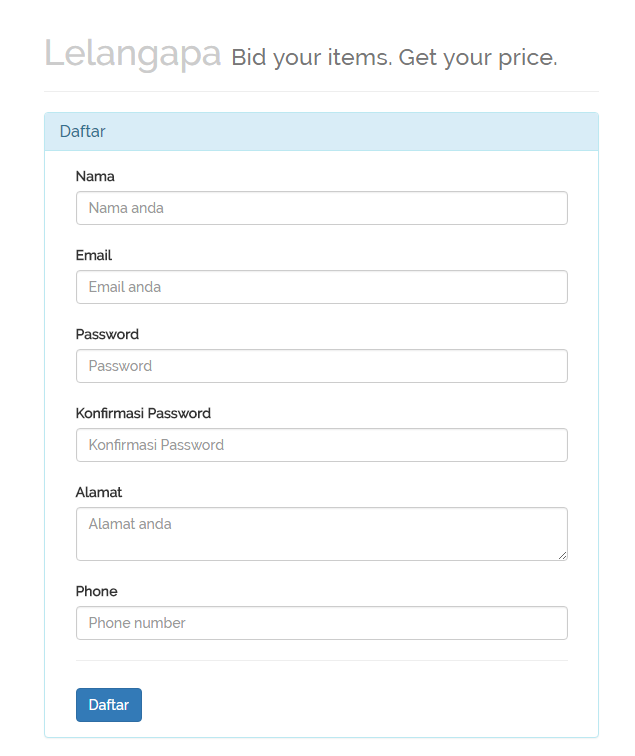
\includegraphics[width=\textwidth]{images/bab4/ui/01-01.png}
    \caption{Halaman antarmuka registrasi}
    \label{ui.01-01}
  \end{figure}
  
\begin{lstlisting}[label=cdbe.01-01,style=php,caption=Kode Sumber Antarmuka Registrasi]
/* 
 * Menampilkan halaman register
 * method : GET 
 */
public function showRegistrationForm(){
	
	return view('auth.register2');
}

/*
 * validator fungsi 
 */
protected function validator(array $data){
	
	return Validator::make($data, [
		'name' => 'required|max:255',
		'email' => 'required|email|max:255|unique:users',
		'password' => 'required|min:6|confirmed',
		'username' => 'required|unique:users|min:5',
		'phone' => 'numeric',
	]);
}

 /*	
  * Dipanggil saat mengklik tombol daftar
  * method : POST 
  */
public function register(Request $request){

				
	/*	validasi data */
	$this->validator($request->all())->validate();

	event(new Registered($user = $this->create($request->all())));

	$this->guard()->login($user);

	/* notify activationService 
	to send activation mail to user's email */
	$this->activationService->sendActivationMail($user);

	return $this->registered($request, $user) ?
	   : redirect($this->redirectPath());
	 
}
	  
	  
\end{lstlisting}
	  
      
      
	% Login ke dalam Sistem
	\subsection{Implementasi Halaman \textit{Login}}
Halaman ini dapat diakses oleh semua pengguna, baik yang belum terdaftar maupun sudah, dengan pengecualian pengguna tidak dalam keadaan sudah \textit{login}. Halaman ini menampilkan form berisi elemen \textit{input} email dan \textit{password}, dan pengguna dapat mengisi lalu mengklik tombol \textit{login}, dan untuk kasus normal dan alternatif dapat dilihat pada tabel spesifikasi kasus penggunaan \ref{uc01.02}.\\
\indent Tidak ada \textit{view logic} dalam halaman ini. Kode sumber implementasi \textit{back-end} dapat dilihat pada kode sumber \ref{cdbe.01-02}.

\begin{lstlisting}[label=cdbe.01-02,style=php,caption=Kode Sumber Antarmuka Registrasi]
public function showLoginForm(){
	/*Menampilkan halaman login
	  Method : GET */
	return view('auth.login2');
}

public function login(Request $request){
	/*	Setelah klik tombol login,
		masuk ke dalam fungsi ini
		Method : POST */
	$this->validateLogin($request);
	return $this->sendLoginResponse($request);
}

\end{lstlisting}

\begin{figure}[H]
	\centering
	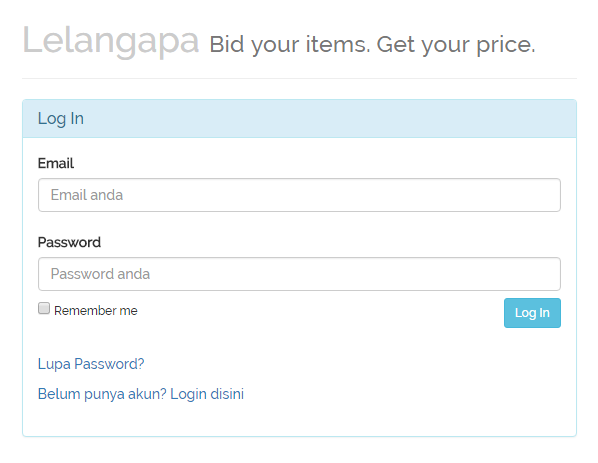
\includegraphics[width=\textwidth]{images/bab4/ui/01-02.png}
	\caption{Halaman Antarmuka }
	\label{ui.01-01}
\end{figure}


	
	
	% Melihat daftar barang yang dilelang
	\subsection{Melihat daftar barang yang dilelang}
Halaman ini hanya dapat diakses oleh pengguna yang sudah terdaftar dan sudah login ke dalam sistem. Halaman ini menampilkan form berisi elemen \textit{input} data diri, dan pengguna dapat mengisi lalu mengklik tombol daftar, dan untuk kasus normal dan alternatif dapat dilihat pada Tabel \ref{uc02.01}.\\
\indent Terdapat view logic khusus pada halaman ini yang ditulis menggunakan Vue dan di\textit{compile} dengan menggunakan webpack, yang akan dicantumkan dalam Kode Sumber \ref{cdv.02-01}. Kode sumber implementasi \textit{back-end} dapat dilihat pada Kode Sumber \ref{cdbe.02-01}.

\begin{lstlisting}[label=cdbe.02-01,style=php,caption=Kode Sumber \textit{Back-end} Melihat Daftar Barang]
/*	file : app/Http/Controllers/HomeController*/
 public function index(){
	 /*	method : GET */
	 
	 /*	variabel berisi id barang 
		yang disort dari tanggal perbaruan
		secara descending */
	 $data['items'] = Item::all()->sortByDesc('created_at');
	 
	 /*	variabel berisi id barang 
		 yang sedang aktif proses lelang
		 menggunakan repository : itemRepository */
	 $data['activebid'] = $this->itemRepository->getActiveItem();
	 

	 return view('pages.general.landing', $data);
 }
\end{lstlisting}

\begin{lstlisting}[label=cdv.02-01,style=htmlcssjs,caption=Kode Sumber Vue Melihat Daftar Barang]
<div>
	 <img :src="imgUrl"  class="img-responsive" />
	 
	 <div class="ribbon" v-if="isFavorited" @click.prevent="unFavorite(item)" >
		 <div class="border-ribbon"></div>
		 <i class="fa fa-heart"></i>
	 </div>
	 
	 <div class="unribbon" v-else @click.prevent="favorite(item)">
		 <div class="border-ribbon"></div>
		 <i class="fa fa-heart-o"></i>
	 </div>
</div>

export default {
    props: ['item', 'favorited'],
    data: function() {
        return {
            isFavorited: '',
            imgUrl : 'http://URL_GAMBAR_DEFAULT'
        }
    },
    mounted() {
        this.isFavorited = this.isFavorite ? true : false;
    },
    created() {
        axios.get("get/img/item/" + this.item)
            .then( response => {
	            if(response.data.replace(/\s+/g, '') != '' ){
	            	var url =  /*rewrite image url*/;
	            	this.imgUrl = url.replace(/\s+/g, '');
	            	console.log(this.imgUrl);
	        	}
    	});
    },
    computed: {
        isFavorite()
        {
            return this.favorited;
        }
    },
    methods: {
        favorite(item){
            axios.post('/ajax/favourite/'+item)
                .then(response => this.isFavorited = true)
        		.catch(response => console.log(response.data));
        	},
        unFavorite(item) {
            axios.post('/ajax/favourite/un/'+item)
                .then(response => this.isFavorited = false)
        		.catch(response => console.log(response.data));
        }
    }
}
\end{lstlisting}

\begin{figure}[H]
	\centering
	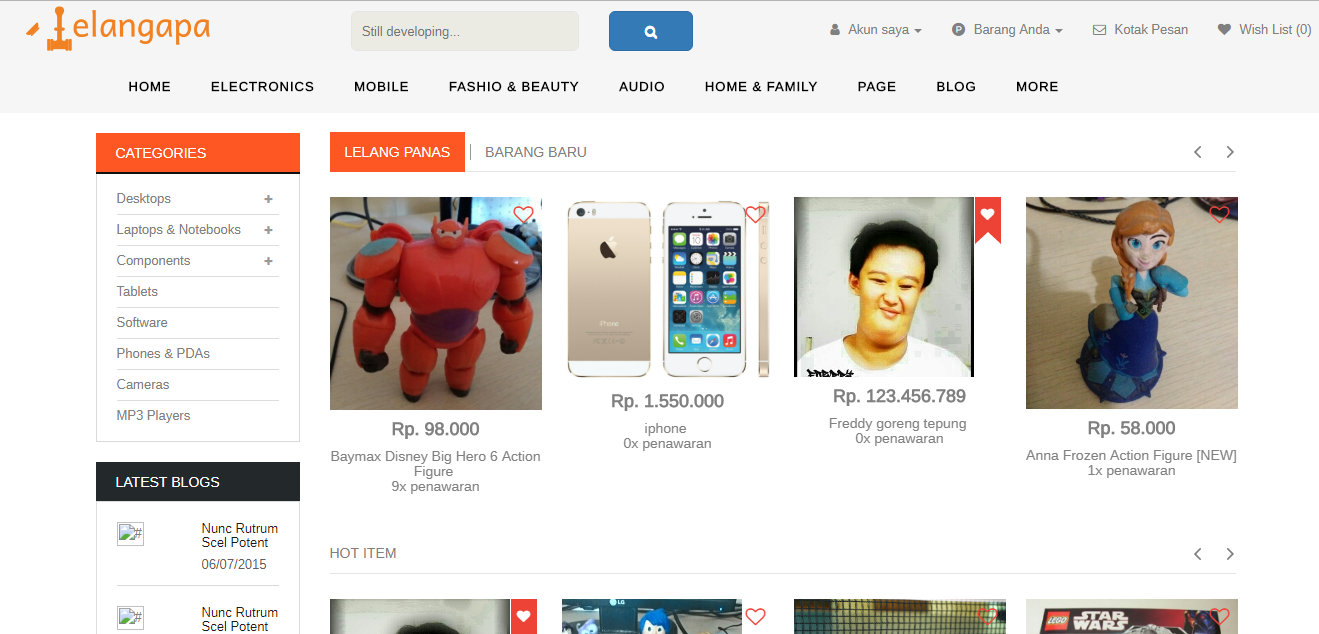
\includegraphics[width=\textwidth]{images/bab4/ui/02-01.png}
	\caption{Halaman antarmuka }
	\label{ui.02-01}
\end{figure}


	% Mencari barang yang diinginkan
	\subsection{Mencari barang yang diinginkan}
	% Menawar/melelang barang
	\subsection{Menawar/melelang barang}
Halaman ini hanya dapat diakses oleh pengguna yang sudah terdaftar. Halaman ini menampilkan halaman informasi barang, dan sebuah elemen \textit{input} harga , dan pengguna dapat mengisi lalu mengklik tombol daftar, dan untuk kasus normal dan alternatif dapat dilihat pada tabel spesifikasi kasus penggunaan \ref{uc02.03}.\\
\indent Sebagai ringkasan dari ketiga logika tersebut, visualisasi pada gambar \ref{cdvis.02-03} akan membantu menggambarkan keseluruhan proses logika secara ringkas. Masing-masing logika tersebut dapat dijabarkan sebagai berikut:
	\begin{enumerate}
		\item Logika \textit{back-end} ditulis menggunakan PHP yang dicantumkan dalam kode sumber \ref{cdjq.02-03}; 
		\item Logika \textit{view} ditulis menggunakan jQuery yang dicantumkan dalam kode sumber \ref{cdjq.02-03}; dan
		\item Logika proses lelang, berjalan diatas socket yang berjalan diatas Node.js dengan bantuan Socket.io yang dicantumkan dalam kode sumber \ref{cdsoc.02-03}
	\end{enumerate}

\begin{figure}[H]
    \centering
    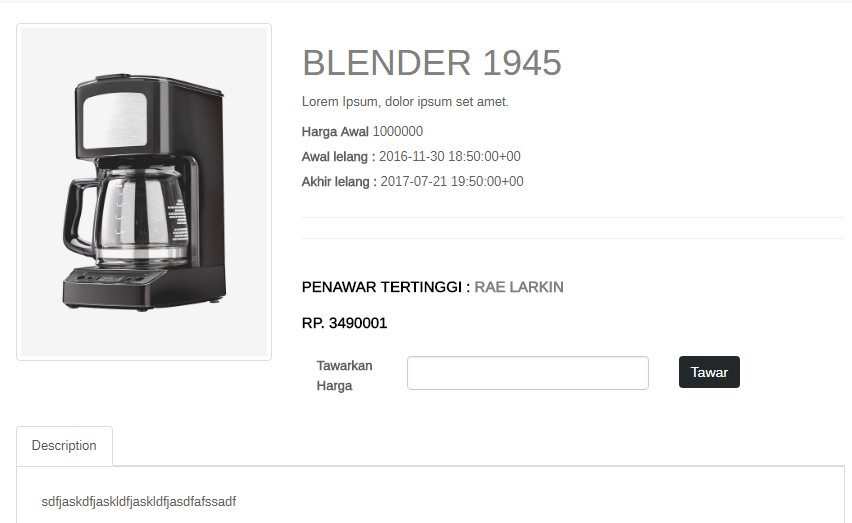
\includegraphics[width=\textwidth]{images/bab4/ui/02-03.png}
    \caption{Halaman Antarmuka  Implementasi Kasus Penggunaan Menawar/melelang barang}
    \label{ui.02-03}
\end{figure}

\begin{lstlisting}[label=cdbe.02-01,style=php,caption=Kode Sumber \textit{Back-end} Menampilkan Halaman Lelang Barang]
/*	file : app/Http/Controllers/ItemController*/
public function show($id){
	/*	method : GET */

	/*	tampilkan halaman */
    $data['item'] = $this->itemRep->find($id);
    
    if($data['item']->bid_status == 1 )
    {
        $data['currentPrice'] = $this->itemRep->getCurrentPrice($id);
    }

    /*	Jika barang yang disubmit sudah selesai/dimenangkan,
    	tambahkan variabel winner ke view */
    if($data['item']->bid_status == -1 && $data['item']->winner_chosen_status)
        $data['winnername'] = User::find($data['item']->id_user)->name;

    /*	tampilkan halaman */
    return view('pages.'.$this->pageFolder.'.detail', $data);
}
\end{lstlisting}


\begin{lstlisting}[label=cdsoc.02-01,style=htmlcssjs,caption=Kode Sumber Logika Lelang (menggunakan Node.js)]
/*	
	file : bidserver_https.js 
	menggunakan dependencies : socketio (ioServer), https, http, fs dan express
*/
socket.on('submitbid', function(bidjson) {

    // parameter (bidjson) adalah JSON yang terdiri dari :
    // id_bidder, id_item, dan harga_bid

    var bidobj = JSON.parse(bidjson);
    biddingAPI.submitBid(bidobj, function(status, result)
    {
      //  status adalah return value
      //  jika status = 1, broadcast ke room
      //  untuk mengupdate pemenang lelang saat tersebut.
      if (status=="1")
      {
          //jika sukses
          var messageObject = {};
          var tokenArray;
            
            // fungsi untuk mengconstruct 
            // return message
          constructBroadcastMsg(messageObject);

            // broadcast ke semua yang 
            // join ke room lelang tersebut.
          io.to(result.item_id_return).emit('bidsuccess', result);
        
      }
      else if (status=="0"){
        // jika gagal, 
        // maka send ke sender bahwa bid failed
        socket.emit('bidfailed', { bidstatus: "failed" });
      }
    });

});
\end{lstlisting}

\begin{lstlisting}[label=cdsoc.02-03,style=htmlcssjs,caption=Kode Sumber Logika UI (menggunakan jQuery)]
// script ini berjalan
// saat tombol Tawar diklik

$('.tawar').click(function()
{
    var penawaran = $('#submitted_price').val();
    var priceNow = $('.priceongoing').html();
    if(penawaran==""){
        alertNoPriceSubmitted();
    }
    else if(penawaran < priceNow ){
        alertInvalidBid();
    }
    else {
        var JSONToSend;
        constructJson(JSONToSend);

        // submit bid ke socket
        socket.emit('submitbid', JSONToSend);

        // tunggu return dari socket
        // jika hasilnya bid failed, maka tampilkan pesan error
        socket.on('bidfailed', function (result) {
            alertFailedBid();
        });

        // jika hasilnya bid sukses,
        // tampilkan pesan sukses (toast)
        // dan render ulang halaman (ubah isi elemen)
        socket.on('bidsuccess', function (result) {
            alertSuccessfulBid();
            renderPageWithNewPrice(result);
        });
    }
});
\end{lstlisting}


	

	% Mendaftarkan barang untuk dilelang
	\subsection{Mendaftarkan Barang untuk Dilelang}
\label{kasus-penggunaan-daftarbarang}
Halaman ini hanya dapat diakses oleh pengguna yang sudah terdaftar dan sudah login ke dalam sistem. Halaman ini menampilkan form berisi elemen \textit{input} informasi barang, dan pengguna dapat mengisi lalu mengklik tombol tambahkan barang, dan untuk kasus normal dan alternatif dapat dilihat pada tabel spesifikasi kasus penggunaan \ref{uc03.01}.\\
\indent Terdapat logika \textit{view} khusus pada implementasi kasus penggunaan ini, karena adanya kebutuhan untuk \textit{upload multiple images} untuk setiap barang dan adanya penggunaan layanan pihak ketiga (AWS Storage Service) sebagai tempat penyimpanan gambar. Kode-kode sumber terkait dengan implementasi kasus penggunaan Mendaftarkan Barang untuk Dilelang adalah sebagai berikut:
	\begin{enumerate}
		\item Logika \textit{back-end} ditulis menggunakan PHP yang dicantumkan dalam kode sumber \ref{cdjq.03-01}; 
		\item Logika \textit{view} ditulis menggunakan jQuery yang dicantumkan dalam kode sumber \ref{cdjq.03-01}; dan
		\item Logika \textit{upload}/\textit{storage} data gambar, yang ditulis menggunakan PHP dicantumka pada kode sumber \ref{cdaws.03-01}
	\end{enumerate} 

  \begin{figure}[H]
    \centering
    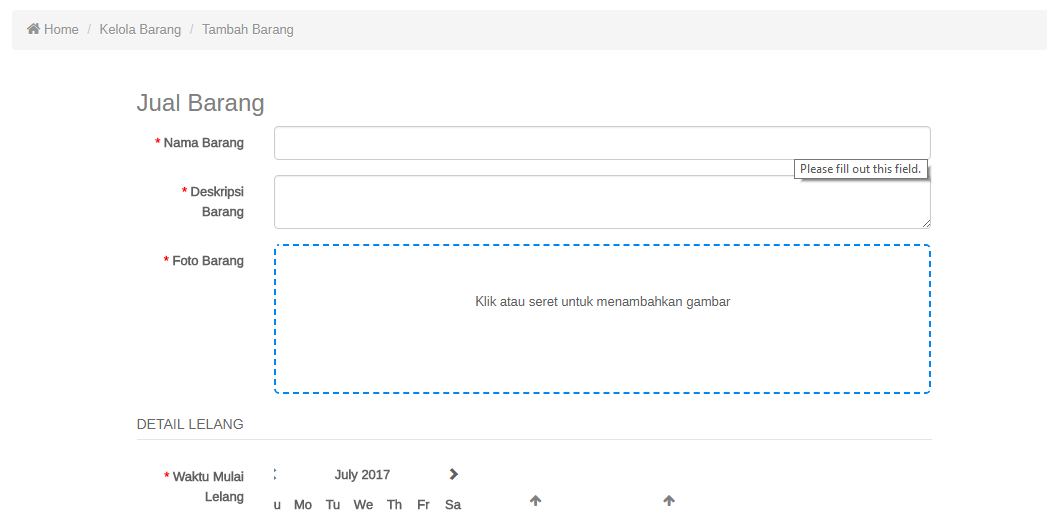
\includegraphics[width=\textwidth]{images/bab4/ui/03-01.png}
    \caption{Halaman antarmuka registrasi}
    \label{ui.01-01}
  \end{figure}

 \begin{lstlisting}[label=cdbe.03-01,style=php,caption=Kode Sumber \textit{Back-end} Mendaftarkan Barang untuk Dilelang]
/*
    Fungsi create() dipanggil untuk menampilkan halaman tambah barang
    Fungsi store() dipanggil saat form di halaman tambah barang diklik
    File : ItemController
*/
public function create(){
    /*  method : GET */
    return view('pages.'.$this->pageFolder.'.create', $data);
}


/*
    Fungsi store() dipanggil oleh ajax lewat jQuery
    untuk memvalidasi dan insert data ke dalam database
*/
public function store(Request $request)
{
    /*  method : POST */
    $unserialize = $this->unserializeForm($request['data']);
    /*  Validating data */
    $validate = Validator::make($unserialize, $this->itemRep->rules(), $this->itemRep->messages());

    if(false){
        /* Jika gagal, return false dan error message 
            ke view
         */
        return ['success'=>false, 'msg' => $validate->messages()];
    }
    else{
        /* 
            Jika sukses, return true 
            dan id barang yang berhasil diinsert
            untuk selanjutnya diproses oleh browser
            untuk upload gambar barang ke URL terpisah.
         */
        return ['success' => true, 'id' =>  10];
    }
}
	  
	  
\end{lstlisting}

\begin{lstlisting}[label=cdjq.03-01,style=php,caption=Kode Sumber \textit{Back-end} Mendaftarkan Barang untuk Dilelang]
/*	
    Fungsi ini berfungsi untuk \textit{update} gambar barang, diteruskan kepada \textit{script} terpisah 
    Pada file : ImageController
    Method : Any
*/
public function uploadItemImage(Request $request){
    //passed here if csrf token is already passed
    $_POST['image'] = $request->file('image');
    $_POST['id_user'] = Auth::user()->id;
    $_POST['ext'] = $request->file('image')->extension();
    
    require ('/home/img/upload-aws.php');

    return $res;
}
\end{lstlisting}


\begin{lstlisting}[label=cdaws.03-01,style=php,caption=Kode Sumber \textit{Back-end} Upload Gambar Barang]
/*	Fungsi ini berfungsi untuk \textit{upload} gambar lewat script terpisah (untuk alasan integrasi data dengan sistem yang dibuat oleh partner tugas akhir)
*/
require 'vendor/autoload.php';

use Aws\S3\S3Client;

$collection = (new MongoDB\Client("mongodb://127.0.0.1:27017"))->lelangkita->itemimages;
if ($_SERVER['REQUEST_METHOD']=='POST'){
        $image = $_POST['image'];
        $userid = $_POST['id_user'];
        $ext = $_POST['ext'];
        $itemid = $_POST['itemid'];
        $isMainImage = false;

        if (isset($_POST['is_main_image']) && !empty($_POST['is_main_image']) && $_POST['is_main_image'] == "true") {
                $isMainImage = true;
        }

        $year = date("Y");
        $month = date("m");
        $date = date("d");
        $unique = uniqid();
        $filename = $userid."_".$unique.".".$ext;
        $path = "img/".$year."/".$month."/".$date."/".$userid;
        $imgpath = $path."/".$filename;

  $decoded_image = base64_decode($image);

  try {
    $s3client = S3Client::factory(array(
      'credentials' => array(
        'key' => 's3\_key\_credentials',
        'secret' => 's3\_secret\_credentials'
      ),
      'profile' => 's3\_profile',
      'region' => 's3\_selected\_server\_regopm'
    ));

    $upload = $s3client->putObject(
      array(
        'Bucket' => 'img-s7.lelangapa.com',
        'Key' => $imgpath,
        'Body'   => $decoded_image,
        'ContentEncoding' => 'base64',
        'ContentType' => 'image/'.$ext,
        'ACL'    => 'public-read'
      )
    );

    $insertToDB = $collection->insertOne([
                'item_id' => $itemid,
                'url' => $imgpath,
                        'is_main_image' => $isMainImage
        ]);

                if ($isMainImage == true) {
                        $indexImageURL = "https://src-api.lelangapa.com/apis/index/submit/image";
                        $headers = array(
                          'Content-Type: application/json'
                        );
                        $post_data = array(
                                "id_item" => $itemid,
                                "main_image_url" => $imgpath
                        );
                        $ch = curl_init();
                        curl_setopt($ch, CURLOPT_URL, $indexImageURL);
                        curl_setopt($ch, CURLOPT_HTTPHEADER, $headers);
                        curl_setopt($ch, CURLOPT_RETURNTRANSFER, 1);
                        curl_setopt($ch, CURLOPT_POST, true);
                        curl_setopt($ch, CURLOPT_POSTFIELDS, json_encode($post_data));
                        curl_setopt($ch, CURLOPT_SSL_VERIFYPEER, FALSE);
                        $indexresult = curl_exec($ch);
                        curl_close($ch);
                }

    if ($upload) {
      $res = array('status' => 'success', 'result' => '1');
                echo "success";
    }
    else {
      $res = array('status' => 'failed', 'result' => '0');
                echo "Failed";
    }
  }
  catch(Exception $e) {
    exit($e->getMessage());
  }
}

\end{lstlisting}
	% Merperbarui informasi barang
	\subsection{Memperbarui Barang}
Halaman ini dapat diakses oleh semua pengguna, baik yang belum terdaftar maupun sudah. Halaman ini menampilkan form berisi elemen \textit{input} data barang yang sebelumnya sudah terisi data-data barang sebelumnya, dan pengguna dapat memperbarui data lalu mengklik tombol Perbarui, dan untuk kasus alternatif dapat dilihat pada tabel spesifikasi kasus penggunaan \ref{uc03.02}.\\
\indent Pada implementasinya, kasus penggunaan ini kurang lebih sama dengan kasus pengunaan Mendaftarkan Barang (subbab \ref{kasus-penggunaan-daftarbarang}) karena adanya penggunaan layanan pihak ketiga (AWS Storage Service) sebagai tempat penyimpanan gambar. Kode-kode sumber terkait dengan implementasi kasus penggunaan Mendaftarkan Barang untuk Dilelang adalah sebagai berikut:
\begin{enumerate}
	\item Logika \textit{back-end} ditulis menggunakan PHP yang dicantumkan dalam kode sumber \ref{cdjq.03-03}; 
	\item Logika \textit{view} ditulis menggunakan jQuery yang dicantumkan dalam kode sumber \ref{cdjq.03-03}; dan
	\item Logika \textit{update image}/\textit{storage} data gambar, yang ditulis menggunakan PHP dicantumkan pada kode sumber \ref{cdaws.03-02}
\end{enumerate} 

\begin{lstlisting}[label=cdbe.03-01,style=php,caption=Kode Sumber \textit{Back-end} Memperbarui Barang]
/*
    Fungsi edit() dipanggil untuk menampilkan halaman perbarui barang
    Fungsi update() dipanggil saat form di halaman update barang disubmit
    File : ItemController
*/
public function edit($id)
{
	/*	method : GET */
    $data['item'] = $this->itemRep->find($id);

    /*	Jika barang sedang aktif lelang,
    	tidak dapat diedit (redirect kembali)	*/
    if($data['item']->bid_status==1){
        return redirect()->back()->with('errorItem','Maaf barang yang sedang dilelang tidak dapat diedit!');
    }
    /*	otorisasi	*/
    if($data['item']->id_user!=Auth::user()->id){
        return redirect()->back()->with('errorItem','Maaf anda tidak terotorisasi!');
    }

    return view('pages.'.$this->pageFolder.'.update', $data);
}


/*
    Fungsi update() dipanggil oleh ajax lewat jQuery
    untuk memvalidasi dan update data ke dalam database
*/
public function store(Request $request)
{
    /*  method : POST */
    $unserialize = $this->unserializeForm($request['data']);
    /*  Validating data */
    $validate = Validator::make($unserialize, $this->itemRep->rules(), $this->itemRep->messages());

    if(false){
        /* Jika gagal, return false dan error message 
            ke view
         */
        return ['success'=>false, 'msg' => $validate->messages()];
    }
    else{
        /* 
            Jika sukses, return true 
            dan id barang yang berhasil diinsert
            untuk selanjutnya diproses oleh browser
            untuk upload gambar barang ke URL terpisah.
         */
        return ['success' => true, 'id' =>  10];
    }
}	  
\end{lstlisting}

\begin{lstlisting}[label=cdjq.03-02,style=htmlcssjs,caption=Kode Sumber \textit{View} Memperbarui Barang]
/*	Fungsi ini berfungsi untuk \textit{update} gambar barang, diteruskan kepada \textit{script} terpisah 
*/
init: function() {
                var submitButton = document.querySelector("#click");
                var myDropzone = this; // closure
                console.log(myDropzone.files.length);
	submitButton.addEventListener("click", function() {
	    swal({
	        text: 'Memperbarui data barang anda...',
	        allowOutsideClick: false,
	        showConfirmButton: false,
	        onOpen: function (){
	            var dataSubmission = $('.submititem').serialize();
	            var startime='&start_time=' + addTimebasedTZ($('#start_time').data().date);
	            var endtime = '&end_time=' + addTimebasedTZ($('#end_time').data().date);
	            dataSubmission += startime;
	            dataSubmission += endtime;
	            $.ajax({
	                type: "POST",
	                url: '{{ route('item.update') }}',
	                data: { _token: '{{csrf_token()}}', data : dataSubmission },
	                success: function( msg ) {
	                    console.log (msg);
	                    if(msg.success == false){
	                        $('.asdf').css('display','block');
	                        $('.asdf').empty();
	                        $.each(msg.msg, function(i, val){
	                            $('.asdf').append(
	                                '<li>'+val+'</li>'
	                            );
	                        });
	                        swal('Oops','Maaf, data anda belum valid. Silahkan cek kembali','error');

	                    }
	                    else{
	                        if(myDropzone.files.length >0){
	                            iditem = msg.id;
	                            myDropzone.processQueue();
	                        }

	                        else{

	                            swal({
	                                title: 'Sukses!',
	                                type:'success',
	                                allowOutsideClick : false,
	                                showConfirmButton : false,
	                                text: "Sukses menambahkan barang!",
	                                timer: 1000
	                            }).then(function () {
	                                document.location = "{{ url('item/') }}" + iditem;
	                            });
	                        }
	                    }

	                }
	            });
	        }
	    });
	});

	this.on("processing", function() {
	    swal('Uploading image..');
	});

	this.on("sending", function(file, xhr, data) {
	    if(iditem != 0){
	        data.append("_token", "{{ csrf_token() }}");
	        data.append("itemid", iditem);
	    }
	});
},
/*	
	saat gagal error gambar,
	bagian fungsi error dipanggil
*/
error: function(file, response) {
    swal({
        title: 'Oops',
        type:'error',
        allowOutsideClick: false,
        showConfirmButton:false,
        text: "Maaf ada kesalahan upload gambar, silahkan upload gambar di halaman edit gambar.",
        timer: 2000
    }).then(function () {
        document.location = "{{ url('item') }}/" + iditem;
    });

},
/*	
	saat sukses update gambar,
	bagian fungsi error dipanggil
*/
success: function(file,done) {
    swal({
        title: 'Sukses!',
        allowOutsideClick: false,
        showConfirmButton:false,
        type:'success',
        text: "Sukses memperbarui barang!",
        timer: 1000
    }).then(function () {
        document.location = "{{ url('item/') }}" + iditem;
    });
}

});

\end{lstlisting}


\begin{lstlisting}[label=cdaws.03-01,style=php,caption=Kode Sumber \textit{Back-end} Upload Gambar Barang]
/*	Fungsi ini berfungsi untuk \textit{upload} gambar lewat script terpisah (untuk alasan integrasi data dengan sistem yang dibuat oleh partner tugas akhir)
*/

use Aws\S3\S3Client;

$collection = (new MongoDB\Client("mongodb://127.0.0.1:27017"))->lelangkita->itemimages;
if ($_SERVER['REQUEST_METHOD']=='POST'){
	constructFilePath();	
	$imgpath = $path."/".$filename;

	$decoded_image = base64_decode($image);

  try {
    $s3client = S3Client::factory(array(
      'credentials' => array(
        'key' => 's3\_key\_credentials',
        'secret' => 's3\_secret\_credentials'
      ),
      'profile' => 's3\_profile',
      'region' => 's3\_selected\_server\_region'
    ));

    $upload = $s3client->putObject(
      array(
        'Bucket' => 'img-s7.lelangapa.com',
        'Key' => $imgpath,
        'Body'   => $decoded_image,
        'ContentEncoding' => 'base64',
        'ContentType' => 'image/'.$ext,
        'ACL'    => 'public-read'
      )
    );

    $insertToDB = $collection->insertOne([
                'item_id' => $itemid,
                'url' => $imgpath,
                        'is_main_image' => $isMainImage
        ]);

                if ($isMainImage == true) {
                        $indexImageURL = "https://src-api.lelangapa.com/apis/index/submit/image";
                        $headers = array(
                          'Content-Type: application/json'
                        );
                        $post_data = array(
                                "id_item" => $itemid,
                                "main_image_url" => $imgpath
                        );
                        $ch = curl_init();
                        curl_setopt($ch, CURLOPT_URL, $indexImageURL);
                        curl_setopt($ch, CURLOPT_HTTPHEADER, $headers);
                        curl_setopt($ch, CURLOPT_RETURNTRANSFER, 1);
                        curl_setopt($ch, CURLOPT_POST, true);
                        curl_setopt($ch, CURLOPT_POSTFIELDS, json_encode($post_data));
                        curl_setopt($ch, CURLOPT_SSL_VERIFYPEER, FALSE);
                        $indexresult = curl_exec($ch);
                        curl_close($ch);
                }
    }
    else {
      $collection->updateOne(
        ['_id' => new \MongoDB\BSON\ObjectID($imageid)],
        ['$set' => array('url' => $imgpath, 'is_main_image' => $isMainImage)]
      );
    }

    if ($upload) {
      $res = array('status' => 'success', 'result' => '1');
                echo "success";
    }
    else {
      $res = array('status' => 'failed', 'result' => '0');
                echo "Failed";
    }
  }
  catch(Exception $e) {
    exit($e->getMessage());
  }
}


\end{lstlisting}

	% Melihat barang yang pernah didaftarkan
	\subsection{Melihat Barang yang Didaftarkan}
Halaman ini hanya dapat diakses oleh pengguna yang sudah terdaftar dan sudah login ke dalam sistem. Halaman ini berisi daftar barang yang pernah didaftarkan pengguna, sesuai dengan spesifikasi kasus penggunaan \ref{uc03.03}.\\
\indent Tidak ada \textit{view logic} ataupun logika \textit{UI} khusus dalam halaman ini. Kode sumber implementasi \textit{back-end} dapat dilihat pada Kode Sumber \ref{cdbe.03-03}.

\begin{lstlisting}[label=cdbe.03-03,style=php,caption=Kode Sumber \textit{Back-end} Melihat Barang yang Pernah Didaftarkan]
/*	
	file : app/Http/Controllers/ItemController
	terkait dengan ItemRepository
*/
 public function index(){
	 /*	method : GET */
	
    $data['items'] = $this->itemRep->getUserItem();
    return view('pages.'.$this->pageFolder.'.index',$data);
}

/*	file : app/Http/Controllers/ItemRepository */
public function getUserItem()
{
    return Auth::user()->item()->orderBy('end_time','desc')->get();
}
\end{lstlisting}

\begin{figure}[H]
	\centering
	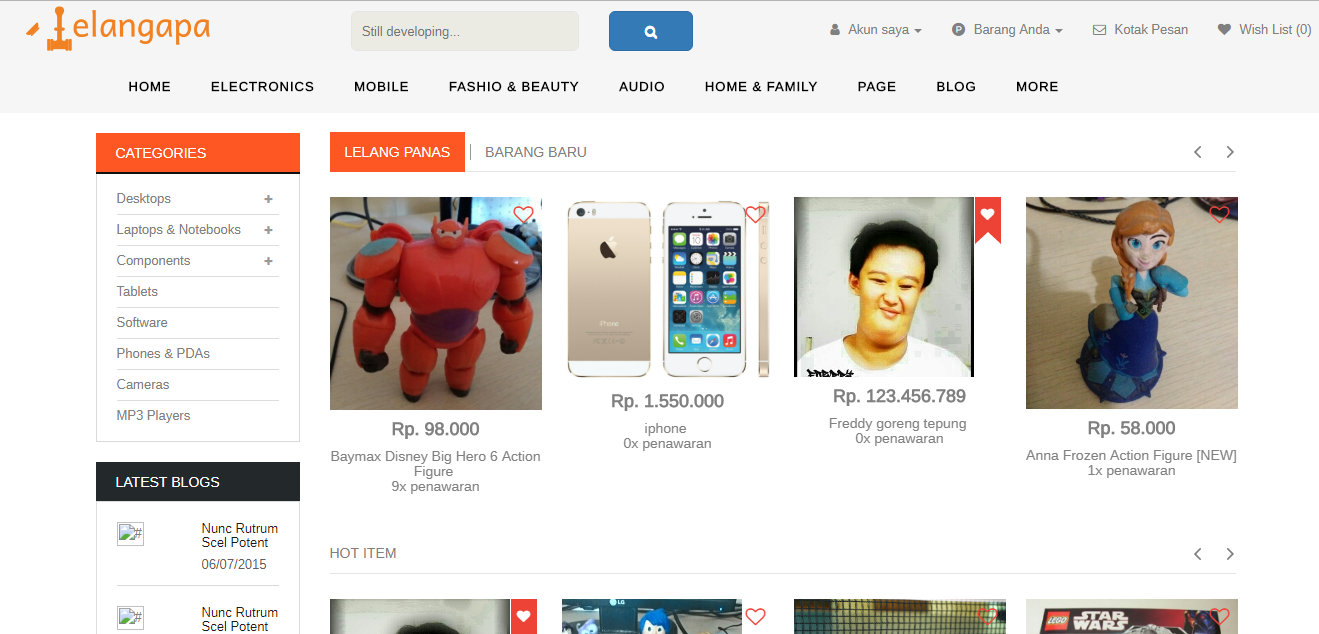
\includegraphics[width=\textwidth]{images/bab4/ui/02-01.png}
	\caption{Halaman antarmuka }
	\label{ui.02-01}
\end{figure}


	% Melihat riwayat harga yang ditawarkan pada barang yang dilelang
	\subsection{Melihat riwayat harga yang ditawarkan pada barang yang dilelang}

	% Melihat review pengguna lainnya
	\subsection{Melihat Review Pengguna Lainnya}


	% Menambahkan review kepada pengguna lainnya
	\subsection{Menambahkan Review}
    Halaman ini hanya dapat diakses oleh pengguna terdaftar yang sudah \textit{login}, dan hanya bisa menambahkan review kepada transaksi yang sudah selesai. Halaman ini menampilkan form \textit{modal} berisi \textit{input} data review, memberikan \textit{rating}. Pengguna dapat mengisi lalu mengklik tombol daftar, untuk kasus alternatif dapat dilihat pada Tabel \ref{uc04.02}.\\
	\indent Terdapat \textit{view logic} khusus dalam halaman ini, karena adanya proses pengecekan terlebih dahulu apakah pengguna sudah pernah memberi \textit{review} sebelumnya. Kode sumber implementasi \textit{back-end} dapat dilihat pada Kode Sumber \ref{cdbe.01-01}.

	\indent Tidak ada logika khusus, hanya logika \textit{back-end} ditulis menggunakan PHP yang dicantumkan dalam Kode Sumber \ref{cdbe.04-02};

\begin{figure}[H]
\centering
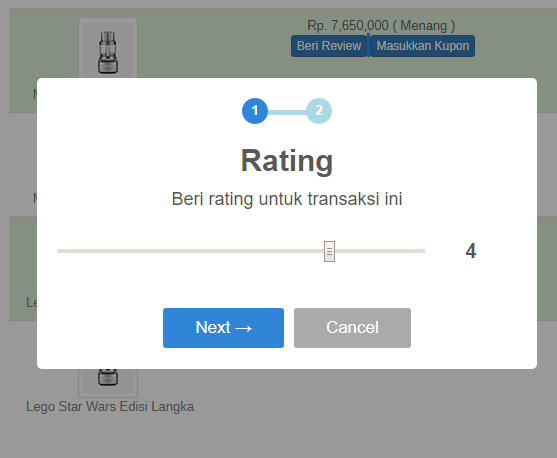
\includegraphics[width=\textwidth]{images/bab4/ui/04-02a.png}
\caption{Halaman Antarmuka Implementasi Menambahkan Review}
\label{ui.04-02a}
\end{figure}


\begin{figure}[H]
\centering
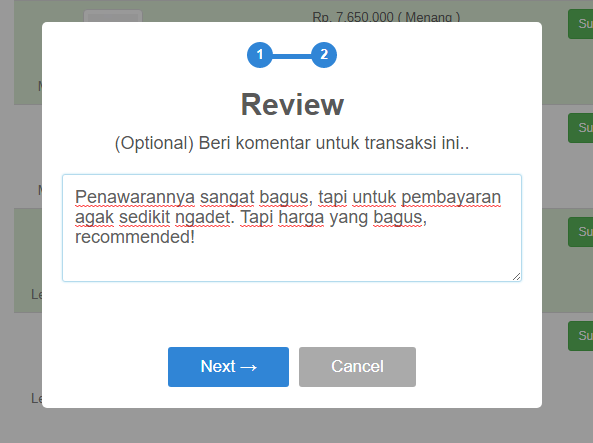
\includegraphics[width=\textwidth]{images/bab4/ui/04-02b.png}
\caption{Halaman Antarmuka Implementasi Menambahkan Review}
\label{ui.04-02b}
\end{figure}

\begin{lstlisting}[label=cdbe.04-02,style=php,caption=Kode Sumber \textit{Back-end} Menambahkan Review]
/*	file : app/Http/Controllers/ReviewController */
/* fungsi ini dieksekusi saat review disubmit */
    
public function submit(Request $request, $idbid)
{
    $informationNeeded = json_decode($request['info']);

    $bid = BidRepository::getBidDetail($idbid);
    $user = $request->user();
    if( !$bid || ($user->id != $bid->id_user && $user->id!= $bid->item->user->id) )
        abort(403);

    return response()
        ->json(
            ReviewRepository::submit($bid, $informationNeeded, $user)
        );
}

/*	file : app/Http/Controllers/ReviewRepository */
public static function submit(Bid $bid, $information, User $user)
{
    $constructArray = [
        'rate' => $information[0],
        'rate_message' => $information[1]
    ];

    $validator = Validator::make($constructArray, self::rule(), self::message());

    if ($validator->fails()) {
        return ['valid'=>false, 'msg'=> $validator->errors() ];
    }

    //stting user yang mau dirate as $user2
    if($user->id == $bid->id_user)
    {
        $user2 = $bid->item->user;
        $isBidder = true;
    }
    else if($user->id == $bid->item->user->id){
        $user2 = $bid->user;
        $isBidder = false;
    }

    $constructQuery = [
        'id_user_rater' => $user->id,
        'nama_user_rater' => $user->name,
        'rate' => $constructArray['rate'],
        'rate_message' => $constructArray['rate_message'],
        'id_item' => $bid->id_item,
        'bid_time' => $bid->bid_time
    ];

//        merge with

    if($isBidder)
        array_merge($constructQuery,
            ['id_user_auctioneer'=> $user2->id, 'nama_user_auctioneer' => $user2->name]);
    else
        array_merge($constructQuery,
            ['id_user_bidder'=> $user2->id, 'nama_user_bidder' => $user2->name]);

    $id = DB::table( $isBidder ? 'ratingauctioneers' : 'ratingbidders')
            ->insertGetId($constructQuery);

    if($id) return ['valid' => true];
        else return ['valid' => false, 'msg' => 'Maaf kesalahan server, silahkan coba lagi'];

    }

/*	file : app/Http/Controllers/BidRepository */
public static function getBidDetail($idbid){
    return Bid::findOrFail($idbid);
}



\end{lstlisting}
	% Melaporkan Barang/Pengguna
	\subsection{Melaporkan Barang/Pengguna}
	% Melihat dan mengirimkan pesan
	\subsection{Mengirimkan pesan}
Halaman ini hanya dapat diakses oleh pengguna yang sudah terdaftar dan masuk/\textit{login} ke dalam sistem. Pada halaman ini terdapat elemen-elemen halaman \textit{chatting} pada umumnya, yaitu elemen \textit{input} pesan, tombol Kirim, dan riwayat beberapa pesan sebelumnya. Spesifikasi kasus penggunaan dapat dilihat pada Tabel \ref{uc04.04}.\\
\indent Terdapat logika \textit{view} dan alur proses khusus dikarenakan sifat pengiriman dan penerimaan pesan yang realtime, sehingga dibangun diatas Node.js dan menggunakan Socket.io. Masing-masing logika tersebut dapat dijabarkan sebagai berikut:
	\begin{enumerate}
		\item Logika \textit{back-end} ditulis menggunakan PHP yang dicantumkan dalam Kode Sumber \ref{cdbe.04-04}; 
		\item Logika \textit{view} ditulis menggunakan jQuery yang dicantumkan dalam Kode Sumber \ref{cdjq.04-04}; dan
		\item Logika proses pengiriman \& penerimaan pesan, berjalan diatas socket yang berjalan diatas Node.js dengan bantuan Socket.io yang dicantumkan dalam Kode Sumber \ref{cdsoc.04-04}
	\end{enumerate}

\begin{figure}[H]
\centering
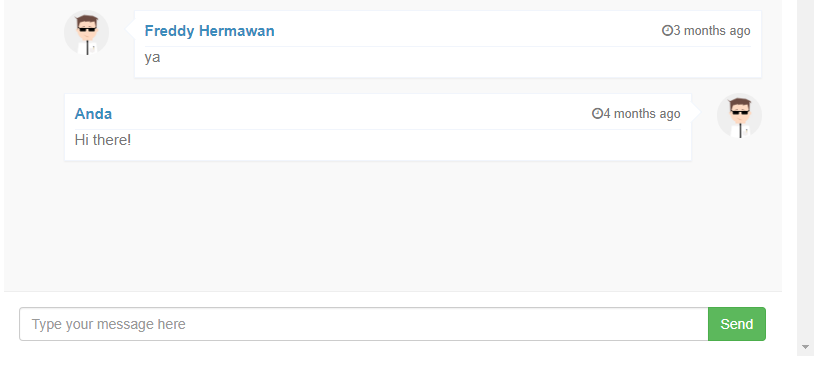
\includegraphics[width=\textwidth]{images/bab4/ui/04-04.png}
\caption{Halaman Antarmuka Implementasi Kasus Penggunaan Mengirimkan Pesan}
\label{ui.04-04}
\end{figure}

\begin{lstlisting}[label=cdbe.04-04,style=php,caption=Kode Sumber \textit{Back-end} Mengirimkan Pesan]
/*	file : app/Http/Controllers/ChatController */
public function chat($id_user)
	/*	method : GET */

    if(intval($id)){
        $data['from'] = Auth::user()->id;
        $data['to'] = $id;
        $data['user'] = User::findOrFail($id);

        if($data['user']){
            return view('pages.user.chat', $data);
        }
    }

    /* 	Jika ada parameter error, 
    	redirect kembali dengan pesan error */
    return redirect('/')->with('error','User yang anda cari tidak dapat ditemukan.');

}
\end{lstlisting}

\begin{lstlisting}[label=cdsoc.04-04,style=htmlcssjs,caption=Kode Sumber Logika View Lelang (menggunakan Node.js)]
/*	
	file : chatserver\_https.js 
	menggunakan dependencies : socketio (ioServer), jwt, https, http, fs dan express
*/
socket.on('join-room', function(room) {
	/*
		fungsi ini dipanggil saat
		pertama kali pengguna membuka halaman chat
		dimana pengguna masuk ke dalam room percakapan
	*/
    var parsedRoom = parseRoom(room);


	/*
		Jika room ini belum pernah dimasuki/ chat perdana
		maka ditambahkan ke tabel joinedroom
	*/
    insertToRoomCollection(roomcollection, parsedRoom, false, function() {
        socket.join(parsedRoom.room);

        // 
        var cb = function(err, chat) {
          if (chat!=[]){
            socket.emit('chathistory', chat);
          }
        };

		/*
			Broadcast 5 percakapan terakhir
			dalam room tersebut
			ke pengguna yang baru saja join room.
		*/
        collection.find({ room : parsedRoom.room }).sort({ sent : -1 }).limit(50).toArray(cb);
    });

});


socket.on('send', function(data) {
	/*
		parameter yang masuk adalah JSON dengan konstruksi berikut :
		{ room: , body : }
	*/

    var msgParse = JSON.parse(data);
    var parsedRoom = parseRoom(msgParse.room);

    //constructing inserting query
    var insertQuery = {
        room : parsedRoom.room,
        sender : parsedRoom.from,
        msg : msgParse.body,
        sent : new Date()
    };

    //insert kedalam database
    collection.insert(insertQuery, function(err, o) {
        var ll = parsedRoom.from.toString();
        if (err) io.to(ll).emit('send-status', { status : false});
        else io.to(ll).emit('send-status', { status : true });
    });

    // update room information
    // bahwa room ini sudah diperbarui
    insertToRoomCollection(roomcollection, parsedRoom, true);

    //broadcast ke user yang tergabung ke room percakapan
    io.to(parsedRoom.room).emit('new-msg', insertQuery);

});

\end{lstlisting}

\begin{lstlisting}[label=cdjq.04-04,style=htmlcssjs,caption=Kode Sumber Logika Pengiriman \& Penerimaan Pesan (menggunakan jQuery)]
var room = '{{ Auth::user()->id }}-{{ $user->id }}';
var prepstat = '{ "room" : "' + room + '", "body" : "';
var closetag ='"}';

/* 
	Masuk ke dalam room
 */
socket.emit('join-room', room);


/* 
	Menerima riwayat perpesanan dan merender pesan-pesan tersebut ke view dengan fungsi bantu appendNewChat()
 */
socket.on('chathistory', function(data){
    console.log(data);
    $(data).each(function(index,value){
        appendNewChat(value);
    });
});

$('.sendMessage').click(function(){
	/*	
		constructing JSON message 
		concate previous statement with message's body
		and close tag
		*/
    var msg = prepstat + $('.body').val() + closetag ;

    /* disable input pesan untuk sementara */
    $(".body").attr("disabled", true);

    /*kirimkan pesan */
    socket.emit('send', msg );

    /* menunggu status pengiriman pesan */
    socket.on('send-status', function(data){
    	/* Jika gagal, enable input pesan dengan tidak menghapus pesan yang belum jadi dikirimkan sebelumnya */
        if(!data.status){
            swal('Oops','Pesan anda tidak dapat terkirim, silahkan coba lagi','error');
        }
        /* Jika sukses, enable input pesan dengan elemen input pesan yang sudah dikosongkan */
        else if(data.status){
            $('.body').val('');
        }

    }, function(){
        $(".body").attr("disabled", false);
    });
});

/* 
	Bagian ini dieksekusi saat ada pesan baru masuk ke dalam room. appendNewChat() adalah fungsi bantu merender view untuk menampilkan pesan baru
 */
socket.on('new-msg', function (value) {
    appendNewChat(value);
});
\end{lstlisting}
	% Melihat kotak pesan
	\subsection{Melihat Kotak Pesan}
	% Memasukkan kupon
	\subsection{Memasukkan kupon}
	
	% Melihat daftar pengguna
	\subsection{Melihat daftar pengguna}
Halaman ini hanya dapat diakses oleh \textit{administrator} yang sebelumnya sudah login. Detail kasus penggunaan dapat dilihat tabel spesifikasi kasus penggunaan \ref{uc05.01}.\\
\indent Tidak ada \textit{view logic} ataupun logika \textit{UI} khusus dalam halaman ini. Kode sumber implementasi \textit{back-end} dapat dilihat pada kode sumber \ref{cdbe.05-01}.

\begin{lstlisting}[label=cdbe.05-01,style=php,caption=Kode Sumber Antarmuka Registrasi]

/** 
 * File : app/Http/Controllers/UserController
 * Menampilkan halaman daftar pengguna
 * langsung diFetch dari base Model User
 * Method : GET
 */
public function user()
{
    $data['data'] = User::paginate(20);
    return view('pages.user.index', $data);
}
\end{lstlisting}
      
  \begin{figure}[H]
    \centering
    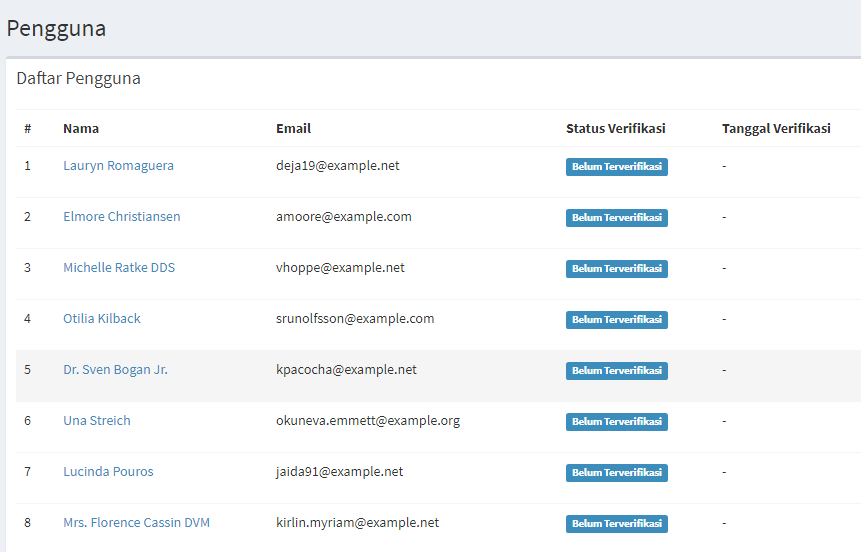
\includegraphics[width=\textwidth]{images/bab4/ui/05-01.png}
    \caption{Halaman Antarmuka Kasus Penggunaan Melihat Daftar Pengguna}
    \label{ui.05-01}
  \end{figure}
      

	% Melihat daftar laporan pengguna
	\subsection{Melihat Daftar Laporan pengguna}
Halaman ini hanya dapat diakses oleh \textit{administrator} yang sebelumnya sudah login. Detail kasus penggunaan dapat dilihat tabel spesifikasi kasus penggunaan \ref{uc05.02}.\\
\indent Tidak ada \textit{view logic} ataupun logika \textit{UI} khusus dalam halaman ini. Kode sumber implementasi \textit{back-end} dapat dilihat pada kode sumber \ref{cdbe.05-02}.

\begin{lstlisting}[label=cdbe.05-02,style=php,caption=Kode Sumber Antarmuka Registrasi]

/** 
 * File : app/Http/Controllers/UserController
 * Menampilkan halaman daftar pengguna
 * langsung diFetch dari base Model User
 * Method : GET
 */
public function user()
{
    $data['data'] = User::paginate(20);
    return view('pages.user.index', $data);
}
\end{lstlisting}
      
%  \begin{figure}[H]
%    \centering
%    \includegraphics[width=\textwidth]{images/bab4/ui/05-02.png}
%    \caption{Halaman Antarmuka Kasus Penggunaan Melihat Daftar Laporan Pengguna}
%    \label{ui.05-02}
% \end{figure}
      

	% Memblock pengguna
	\subsection{Memblock pengguna}
Halaman ini hanya dapat diakses oleh \textit{administrator} yang sebelumnya sudah login. Detail kasus penggunaan dapat dilihat tabel spesifikasi kasus penggunaan \ref{uc05.02}.\\
\indent Tidak ada \textit{view logic} ataupun logika \textit{UI} khusus dalam halaman ini. Kode sumber implementasi \textit{back-end} dapat dilihat pada kode sumber \ref{cdbe.05-02}.

\begin{lstlisting}[label=cdbe.05-02,style=php,caption=Kode Sumber Antarmuka Registrasi]

/** 
 * File : app/Http/Controllers/UserController
 * Menampilkan halaman daftar pengguna
 * langsung diFetch dari base Model User
 * Method : GET
 */
public function user()
{
    $data['data'] = User::paginate(20);
    return view('pages.user.index', $data);
}
\end{lstlisting}
      
%  \begin{figure}[H]
%    \centering
%    \includegraphics[width=\textwidth]{images/bab4/ui/05-02.png}
%    \caption{Halaman Antarmuka Kasus Penggunaan Melihat Daftar Laporan Pengguna}
%    \label{ui.05-02}
%  \end{figure}

	% Menambahkan voucher
	\subsection{Menambahkan voucher}
Halaman ini hanya dapat diakses oleh \textit{administrator} yang sebelumnya sudah login. Halaman ini menampilkan form berisi elemen \textit{input} informasi voucher, dan setelah selesai lalu mengklik tombol Tambahkan Voucher, dan untuk kasus alternatif dapat dilihat pada tabel spesifikasi kasus penggunaan \ref{uc06.01}.\\
\indent Tidak ada \textit{view logic} ataupun logika \textit{UI} khusus dalam halaman ini. Kode sumber implementasi \textit{back-end} dapat dilihat pada kode sumber \ref{cdbe.06-01}.

\begin{lstlisting}[label=cdbe.06-01,style=php,caption=Kode Sumber Antarmuka Registrasi]

/** File : app/Http/Controllers/CouponController
 * Menampilkan halaman tambah kupon
 * Method : GET
 */
public function create()
{
    $data['user'] = $this->userRepository->checkbox();
    return view('pages.coupon.create',$data);
}

/**
 * Store data kupon yang dimasukkan
 * fungsi ini dijalankan ketika form disubmit
 * terkait dengan CouponRepository
 */

public function store(Request $request)
{
    $data = $request->all();
    $data['limit_usages'] = $data['usages'];
    $ss = $this->couponRepository->storeCoupon($data);

    if($ss) return redirect('coupon')->with('success',true);
    else return redirect('coupon')->with('success',false);
}


/**
 * File CouponRepository
 */
public function storeCoupon($data)
{
	/* Menggunakan base model Laravel */
	/* return status store data ke dalam database */
    return Coupon::create($data);
}  
\end{lstlisting}
	  
      \begin{figure}[H]
        \centering
        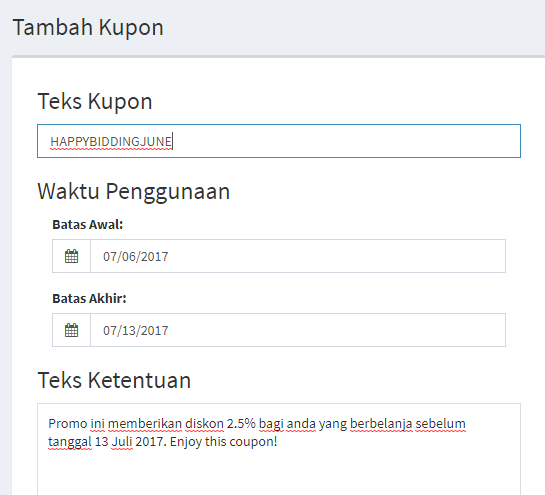
\includegraphics[width=\textwidth]{images/bab4/ui/06-01.png}
        \caption{Halaman Antarmuka Kasus Penggunaan Menambahkan Voucher}
        \label{ui.01-01}
      \end{figure}
      

	% Melihat daftar voucher
	\subsection{Melihat daftar voucher}
Halaman ini hanya dapat diakses oleh \textit{administrator} yang sebelumnya sudah login. Detail kasus penggunaan dapat dilihat Tabel \ref{uc06.02}.\\
\indent Tidak ada \textit{view logic} ataupun logika \textit{UI} khusus dalam halaman ini. Kode sumber implementasi \textit{back-end} dapat dilihat pada Kode Sumber \ref{cdbe.06-02}.

\begin{lstlisting}[label=cdbe.06-02,style=php,caption=Kode Sumber Antarmuka Registrasi]

/** File : app/Http/Controllers/CouponController
 * Menampilkan halaman daftar kupon
 * tidak terkait dengan CouponRepository
 * langsung diFetch dari base Model Coupon
 * Method : GET
 */

public function index()
{
    $data['data'] = Coupon::orderBy('activedate', 'desc')->paginate(20);
    return view('pages.coupon.index', $data);

}
\end{lstlisting}
      
  \begin{figure}[H]
    \centering
    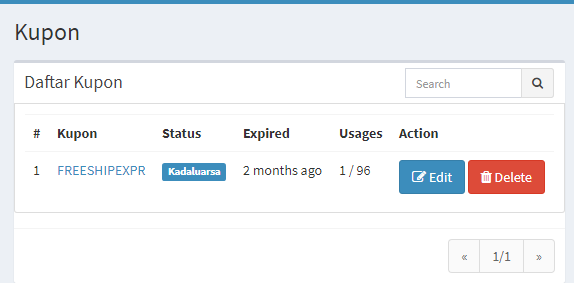
\includegraphics[width=\textwidth]{images/bab4/ui/06-02.png}
    \caption{Halaman Antarmuka Kasus Penggunaan Melihat Daftar Voucher}
    \label{ui.06-02}
  \end{figure}
      

	% Memperbarui Voucher
	\subsection{Memperbarui kupon}
Halaman ini hanya dapat diakses oleh \textit{administrator} yang sebelumnya sudah login. Detail kasus penggunaan dapat dilihat Tabel \ref{uc06.03}.\\
\indent Tidak ada \textit{view logic} ataupun logika \textit{UI} khusus dalam halaman ini. Kode sumber implementasi \textit{back-end} dapat dilihat pada Kode Sumber \ref{cdbe.06-03}.

\begin{lstlisting}[label=cdbe.06-03,style=php,caption=Kode Sumber Implementasi \textit{Back-end} Kasus Penggunaan Memperbarui kupon]

/** File : app/Http/Controllers/CouponController
 * Menampilkan halaman perbarui kupon
 * Method : GET
 */
public function edit($id)
{
    try{
        $data['user'] = $this->userRepository->checkbox();
        $data['coupon'] = $this->couponRepository->find($id);
        return view('pages.coupon.edit', $data);
    }
    catch (\Exception $e){
        abort(403);
    }
}
/**
 * Update data kupon yang dimasukkan
 * fungsi ini dijalankan ketika form di halaman edit  kupon disubmit
 * terkait dengan CouponRepository
 */

public function update(Request $request, $id)
{

    $data = $request->all();
    if($this->couponRepository->update($id, $data)){
        return redirect('coupon')->with('success','Sukses memperbarui kupon!');
    }
    else return redirect('coupon')->with('error','Mohon maaf, gagal memperbarui kupon. Silahkan coba lagi');
}


/**
 * File CouponRepository
 */
public function update($id, $data)
{
    $coupon = $this->find($id);
    return $coupon->update($data);

}
\end{lstlisting}
	  
%  \begin{figure}[H]
%    \centering
%    \includegraphics[width=\textwidth]{images/bab4/ui/06-03.png}
%    \caption{Halaman Antarmuka Kasus Penggunaan Memperbarui kupon}
%    \label{ui.01-01}
%  \end{figure}
      

	